\section{本論}
\subsection{課題1}
\subsubsection{結果}
以下の計測方法で得られた識別精度を表\ref{table:1}から表\ref{table:4}にそれぞれ示す。
全ての計測方法において、それぞれのデータで最も精度が高かったものを\textcolor{red}{赤く}
表示している。
\begin{itemize}
  \item k最近傍法(k=5):kNN5
  \item 線形サポートベクトルマシン:linearSVM
  \item 非線形サポートベクトルマシン(RBFカーネル):nonlinearSVM
  \item ランダムフォレスト:randomForest
\end{itemize}

\begin{table}[hbtp]
  \begin{tabular}{ccc}
    \begin{minipage}[t]{0.24\hsize}
      \centering
      \caption{knn5の結果}
      \label{table:1}
      \begin{tabular}{|c|c|}
        \hline
        data & 平均精度\\
        \hline
        1 & \textcolor{red}{1.000}   \\
        2 & 0.987  \\
        3 & \textcolor{red}{0.997}  \\
        4 & 0.753  \\
        5 & \textcolor{red}{0.963}  \\
        \hline
      \end{tabular}
    \end{minipage}
    \begin{minipage}[t]{0.24\hsize}
      \centering
      \caption{linearSVMの結果}
      \label{table:2}
      \begin{tabular}{|c|c|}
        \hline
        data & 平均精度\\
        \hline
        1 & \textcolor{red}{1.000}  \\
        2 & \textcolor{red}{0.990}  \\
        3 & 0.460  \\
        4 & 0.443  \\
        5 & 0.909  \\
        \hline
      \end{tabular}
    \end{minipage}
    \begin{minipage}[t]{0.24\hsize}
      \centering
      \caption{nonlinearSVMの結果}
      \label{table:3}
      \begin{tabular}{|c|c|}
        \hline
        data & 平均精度\\
        \hline
        1 & \textcolor{red}{1.000}  \\
        2 & \textcolor{red}{0.990}  \\
        3 & \textcolor{red}{0.997}  \\
        4 & \textcolor{red}{0.800}  \\
        5 & 0.450  \\
        \hline
      \end{tabular}
    \end{minipage}
    \begin{minipage}[t]{0.24\hsize}
      \centering
      \caption{randomForestの結果}
      \label{table:4}
      \begin{tabular}{|c|c|}
        \hline
        data & 平均精度\\
        \hline
        1 & \textcolor{red}{1.000}  \\
        2 & 0.983  \\
        3 & \textcolor{red}{0.997}  \\
        4 & 0.770  \\
        5 & 0.933  \\
        \hline
      \end{tabular}
    \end{minipage}
  \end{tabular}
\end{table}
以下の、図\ref{graph:1}はdata1で線形サポートベクトルマシン、
図\ref{graph:2}はdata2で線形サポートベクトルマシン、
図\ref{graph:3}はdata3でk再近傍法、
図\ref{graph:4}はdata4で非線形サポートベクトルマシンを使った際のグラフ
である。

\begin{figure}[htbp]
  \begin{minipage}[t]{0.24\hsize}
    \centering
    \caption{Data1\_linearSVM}
    \label{graph:1}
    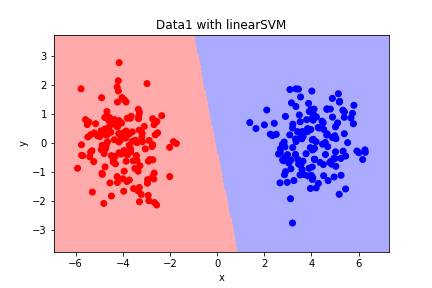
\includegraphics[keepaspectratio, scale=0.3]{fig_20210629132055/Data1_linearSVM.png}
  \end{minipage}
  \begin{minipage}[t]{0.24\hsize}
    \centering
    \caption{Data2\_linearSVM}
    \label{graph:2}
    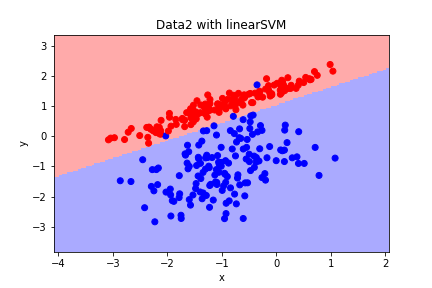
\includegraphics[keepaspectratio, scale=0.3]{fig_20210629132055/Data2_linearSVM.png}
  \end{minipage}
  \begin{minipage}[t]{0.24\hsize}
    \centering
    \caption{Data3\_kNN5}
    \label{graph:3}
    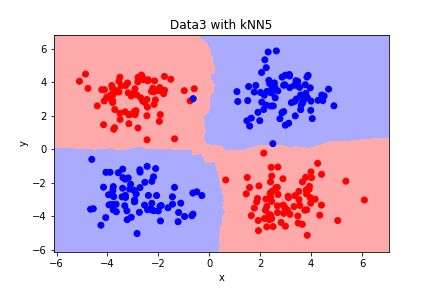
\includegraphics[keepaspectratio, scale=0.3]{fig_20210629132055/Data3_kNN5.png}
  \end{minipage}
  \begin{minipage}[t]{0.24\hsize}
    \centering
    \caption{Data4\_nonlinearSVM}
    \label{graph:4}
    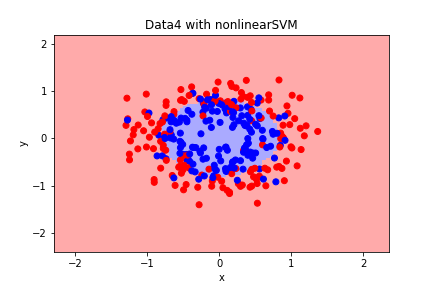
\includegraphics[keepaspectratio, scale=0.3]{fig_20210629132055/Data4_nonlinearSVM.png}
  \end{minipage}
\end{figure}

\subsubsection{考察}
\begin{itemize}
  \item そのデータに対して適していると思われる手法とその理由
  \begin{itemize}
    \item[data1] 適していると思われる手法は、線形サポートベクトルマシンである。
    理由は、過学習を避けるために単純なモデルである線形サポートベクトルマシンから試していくと、
    線形サポートベクトルマシンの時点で精度が「1.000」となっており、十分な精度があるためである。
    \item[data2] 適していると思われる手法は、線形サポートベクトルマシンである。
    理由は、data1の時と同じように単純なモデルから試していくと、線形サポートベクトルマシンの時点で
    、精度が「0.990」となっており、十分な精度があるためである。
    \item[data3] 適していると思われる手法は、k再近傍法(k=5)である。
    理由は、data1の時と同じように単純なモデルから試していくと、
    線形サポートベクトルマシンでは精度が「0.460」となり、精度が悪い。そのため、
    次に単純なモデルであるk再近傍法(k=5)を試すと、精度が「0.997」となり、十分な精度があるため
    、適していると思われる。
    \item[data4] 適していると思われる手法は、非線形サポートベクトルマシンである。
    理由は、data1の時と同じように単純なモデルから試していくと、非線形サポートベクトルマシン
    は、精度が「0.443」となり、精度が悪い。次に、単純なモデルであるk再近傍法(k=5)の精度は、
    「0.753」となり、精度がやや悪い。次に、非線形サポートベクトルマシンとランダムフォレスト
    の精度を見ると、それぞれ精度が「0.800」,「0.770」となり、非線形サポートベクトルマシン
    の精度が一番高くなるため、適していると思われる。
    \item[data5] 適していると思われる手法は、k再近傍法(k=5)である。
    理由は、data1の時と同じように単純なモデルから試していくと、線形サポートベクトルマシン
    の精度は「0.909」となり、精度は十分といえない。次に、単純なモデルであるk再近傍法(k=5)
    の精度は、「0.963」となり、十分な精度があるため、適していると思われる。
  \end{itemize}
  \item この結論が得られたのはデータにどのような性質があるからか
  \begin{itemize}
    \item[data1] 図\ref{graph:1}を見てわかる通り、データが線形分離可能であるため、
    線形サポートベクトルマシンが適しているとなった。
    \item[data2] 図\ref{graph:2}を見ると、data1と同じくデータは線形分離可能であるため、
    線形サポートベクトルマシンが適しているとなった。
    \item[data3] 図\ref{graph:3}を見ると、データは線形分離不可能であるため、
    線形サポートベクトルマシンの精度は悪い。しかし、同じクラスのデータ同士で固まっている
    ため、次に単純なモデルであるk再近傍法(k=5)が適しているとなった。
    \item[data4] 図\ref{graph:4}を見ると、データは線形分離不可能であるため、
    線形サポートベクトルマシンの精度は悪い。そして、赤のクラスのデータに囲われるように
    青のクラスのデータが存在しており、それらの距離が近いため、k再近傍法も精度は悪い。
    非線形サポートベクトルマシンの精度は比較的に高かったことから、
    データを多次元化すると、ソフトマージンでの線形分離が可能になったと考えられる。
    \item[data5] k再近傍法(k=5)の精度が高かったことから、一つのデータの近傍5個のデータ
    で同じクラスのデータが多かったと考えられる。
  \end{itemize}
\end{itemize}
\clearpage


\subsection{課題2}
\subsubsection{結果}
以下の表\ref{table:5}に、課題1でとりあげた4つの手法をData5に適用した時の、
学習にかかった時間、テストにかかった時間、平均精度をそれぞれ示す。

\begin{table}[hbtp]
  \centering
  \caption{それぞれの手法でのデータ5の結果}
  \label{table:5}
  \begin{tabular}{|c|c|c|c|}
    \hline
    手法 & 学習にかかった時間 & テストにかかった時間 & 平均精度\\
    \hline
    k最近傍法(k=5) & 0.00796 [秒] & 0.08403 [秒] &  0.963 \\
    線形サポートベクトルマシン & 0.12577 [秒] & 0.00114 [秒] &  0.909  \\
    非線形サポートベクトルマシン & 0.46725 [秒] & 0.05381 [秒] &  0.450 \\
    ランダムフォレスト & 0.17586 [秒] & 0.00995 [秒] &  0.933 \\
    \hline
  \end{tabular}
\end{table}

\subsubsection{考察}
\begin{itemize}
  \item 非線形サポートベクトルマシンは、他の手法に比べて、学習にかかった時間とテストにかかった時間
  の両方がともに長い傾向に見られる。これは、非線形サポートベクトルマシンが多次元のデータを扱っているため
  に時間がかかっていると考えられる。
  \item 線形サポートベクトルマシンとランダムフォレストの
  学習にかかった時間はk再近傍法(k=5)に比べて、長くなる傾向が見られる。しかし、テストにかかった時間
  では、反対の結果となりk再近傍法(k=5)の方が長くなっている。
  これは、線形サポートベクトルマシンやランダムフォレストでは、モデルを適切に学習することが精度に
  繋がっているため、時間がかかるものの、
  k再近傍法では、テスト時に
  近傍点を見つけるため、新しいデータと既存の全データとの距離を知る必要がある。
  そのため、k再近傍法ではテストにかかる時間の方が長くなる。
  また、k再近傍法では、上記の処理がメインであるため、
  準備や学習にはほとんど時間がかからない。
\end{itemize}



\clearpage
\subsection{課題3}
\subsubsection{課題3-1}
非線形サポートベクトルマシンのパラメータを以下の図\ref{graph:5}から図\ref{graph:7}のように
して実行したところ、以下の図\ref{graph:8}から図\ref{graph:9}のような結果が得られた。
特にパラメータセット2とパラメータセット3は、課題1で得られた最良の精度を超える精度となった。

\begin{figure}[htbp]
  \begin{minipage}[t]{0.33\hsize}
    \centering
    \caption{パラメータセット1}
    \label{graph:5}
    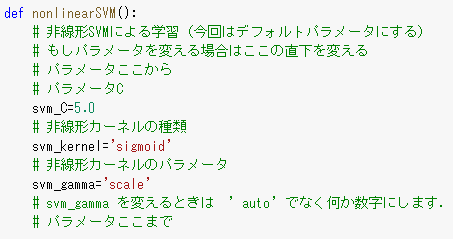
\includegraphics[keepaspectratio, scale=0.5]{3-1-1r.PNG}
  \end{minipage}
  \begin{minipage}[t]{0.33\hsize}
    \centering
    \caption{パラメータセット2}
    \label{graph:6}
    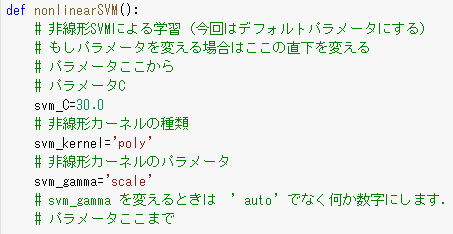
\includegraphics[keepaspectratio, scale=0.5]{3-1-2r.PNG}
  \end{minipage}
  \begin{minipage}[t]{0.33\hsize}
    \centering
    \caption{パラメータセット3}
    \label{graph:7}
    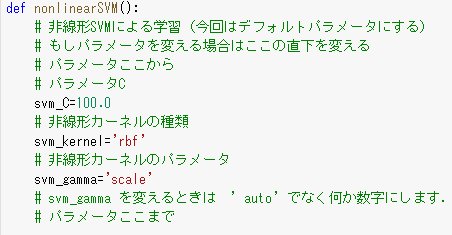
\includegraphics[keepaspectratio, scale=0.5]{3-1-3r.PNG}
  \end{minipage}
  \begin{minipage}[t]{0.33\hsize}
    \centering
    \caption{パラメータセット1の結果}
    \label{graph:8}
    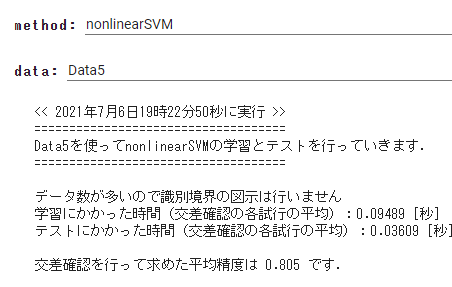
\includegraphics[keepaspectratio, scale=0.5]{3-1-1.PNG}
  \end{minipage}
  \begin{minipage}[t]{0.33\hsize}
    \centering
    \caption{パラメータセット2の結果}
    \label{graph:9}
    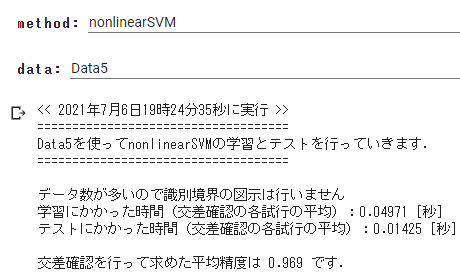
\includegraphics[keepaspectratio, scale=0.5]{3-1-2.PNG}
  \end{minipage}
  \begin{minipage}[t]{0.33\hsize}
    \centering
    \caption{パラメータセット3の結果}
    \label{graph:10}
    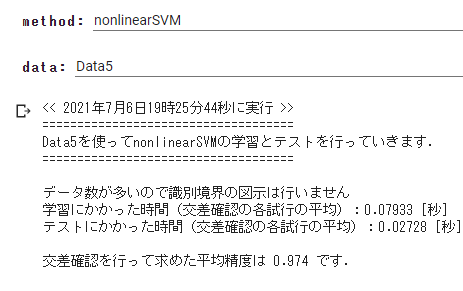
\includegraphics[keepaspectratio, scale=0.5]{3-1-3.PNG}
  \end{minipage}
\end{figure}

パラメータと精度を表にすると、以下の表\ref{table:6}のようになった。
\begin{table}[hbtp]
  \centering
  \caption{それぞれのパラメータセットでの精度}
  \label{table:6}
  \begin{tabular}{|c|c|c|c|c|}
    \hline
    パラメータセット&パラメータC & 非線形カーネルの種類 & 非線形カーネルのパラメータ & 平均精度\\
    \hline
    1&5.0 & sigmoid & scale &  0.805 \\
    2&30.0 & poly & scale &  0.969  \\
    3&100.0 & rbf & scale &  0.974 \\
    \hline
  \end{tabular}
\end{table}
\clearpage
\subsubsection{課題3-2}
\subsubsection{結果}
決定木の最大深さ1,5,10にそれぞれ変えて実行したところ、表\ref{table:7}のような結果となった。
また、以下の図\ref{graph:11}から図\ref{graph:13}のような識別境界が得られた。

\begin{table}[hbtp]
  \centering
  \caption{木の最大深さごとの精度}
  \label{table:7}
  \begin{tabular}{|c|c|}
    \hline
    木の最大深さ&平均精度\\
    \hline
    1&0.540 \\
    5&0.733  \\
    10&0.670  \\
    \hline
  \end{tabular}
\end{table}
\begin{figure}[htbp]
  \begin{minipage}[t]{0.33\hsize}
    \centering
    \caption{木の最大深さ1の識別境界}
    \label{graph:11}
    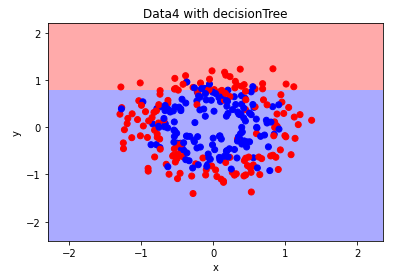
\includegraphics[keepaspectratio, scale=0.5]{3-2-1.PNG}
  \end{minipage}
  \begin{minipage}[t]{0.33\hsize}
    \centering
    \caption{木の最大深さ5の識別境界}
    \label{graph:12}
    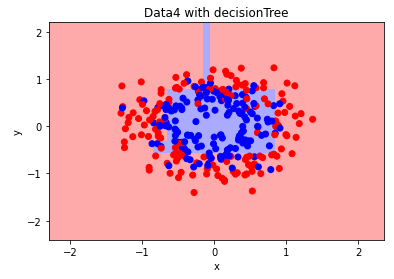
\includegraphics[keepaspectratio, scale=0.5]{3-2-5.PNG}
  \end{minipage}
  \begin{minipage}[t]{0.33\hsize}
    \centering
    \caption{木の最大深さ10の識別境界}
    \label{graph:13}
    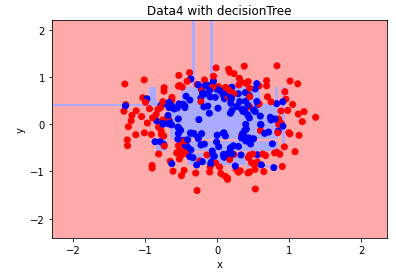
\includegraphics[keepaspectratio, scale=0.5]{3-2-10.PNG}
  \end{minipage}
\end{figure}
\subsubsection{考察}
\begin{itemize}
  \item 木の最大深さが1の時に、図\ref{graph:11}のようになったのは、分岐が二つしかないため、yが
  ある値n以上なら赤
  、それ以外なら青のように分けられたと考えられる。
  \item 木の最大深さが5から10になった時に、精度が下がってしまったのは、分岐が多くなったために、外れ値を
  条件にしてしまう「過学習」が起こったためだと考えられる。
\end{itemize}
\clearpage

\subsubsection{課題3-3}
「ConvergenceWarning」は線形サポートベクトルマシンを使っている際に出力される。
線形サポートベクトルマシンは2次元線形分離することで識別するが、その線形分離の線が
1意に収束しない時に、「ConvergenceWarning」となる。
